\documentclass[tikz,border=10pt]{standalone}
\usetikzlibrary{calc, decorations.markings}

\begin{document}
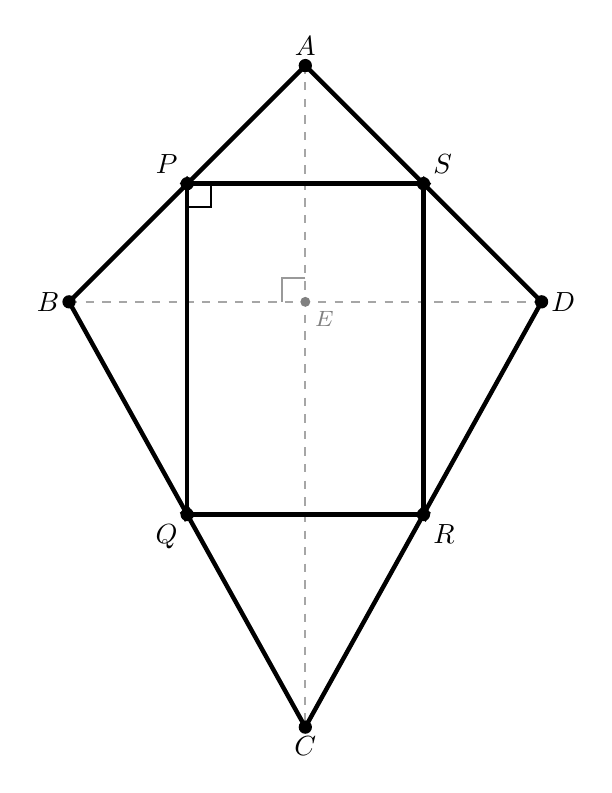
\begin{tikzpicture}[>=stealth, scale=1.2]

  % Styles for midpoint markers (double lines to indicate midpoints)
  \tikzset{
    midtick/.style={
      postaction={decorate},
      decoration={
        markings,
        mark=at position 0.5 with {\draw[thick] (-1.5pt,-2pt) -- (-1.5pt,2pt); \draw[thick] (1.5pt,-2pt) -- (1.5pt,2pt);}
      }
    }
  }

  % 1. Define Main Kite Vertices
  \coordinate (A) at (0,4);
  \coordinate (B) at (-2.5,1.5);
  \coordinate (D) at (2.5,1.5);
  \coordinate (C) at (0,-3);
  \coordinate (E) at (0,1.5); % Diagonal intersection

  % 2. Compute Midpoints using the calc library
  \coordinate (P) at ($(A)!0.5!(B)$);
  \coordinate (Q) at ($(B)!0.5!(C)$);
  \coordinate (R) at ($(C)!0.5!(D)$);
  \coordinate (S) at ($(D)!0.5!(A)$);

  % --- DRAWING LINES ---
  % Outer Kite Diagonals (Structural reference lines)
  \draw[thick, dashed, gray!70] (A) -- (C);
  \draw[thick, dashed, gray!70] (B) -- (D);

  % Outer Kite Sides with Midpoint Division Markings
  \draw[ultra thick, midtick] (A) -- (B);
  \draw[ultra thick, midtick] (B) -- (C);
  \draw[ultra thick, midtick] (C) -- (D);
  \draw[ultra thick, midtick] (D) -- (A);

  % Inner Rectangle Boundary (No fill)
  \draw[ultra thick, black!50!black] (P) -- (Q) -- (R) -- (S) -- cycle;

  % --- PERPENDICULAR RIGHT ANGLE MARKERS ---
  % Right angle at the diagonal intersection (E)
  \draw[thick, gray!80] ($(E)+(0,0.25)$) -- ($(E)+(-0.25,0.25)$) -- ($(E)+(-0.25,0)$);

  % Right angle at Varignon vertex P
  % Calculated dynamically along the directions of PS and PQ
  \draw[thick, black!50!black]
    ( $(P)!0.25cm!(S)$ ) --
    ( $($(P)!0.25cm!(S)$) + ($(P)!0.25cm!(Q)$) - (P)$ ) --
    ( $(P)!0.25cm!(Q)$ );

  % --- DOTS AND LABELS ---
  % Kite Vertices
  \fill (A) circle (2pt) node[above] {$A$};
  \fill (B) circle (2pt) node[left] {$B$};
  \fill (C) circle (2pt) node[below] {$C$};
  \fill (D) circle (2pt) node[right] {$D$};
  \fill[gray] (E) circle (1.5pt) node[below right, font=\footnotesize, text=gray] {$E$};

  % Midpoint Vertices
  \fill[black!50!black] (P) circle (2pt) node[above left] {$P$};
  \fill[black!50!black] (Q) circle (2pt) node[below left] {$Q$};
  \fill[black!50!black] (R) circle (2pt) node[below right] {$R$};
  \fill[black!50!black] (S) circle (2pt) node[above right] {$S$};

\end{tikzpicture}
\end{document}
